%%%%%%%%%%%%%%%%%%%%%%%%%%%%%%%%%%%%%%%%%%%%%%%%%%%%%%%%%%%%%%%%%%%%%
% In English:
%    This is a Latex template for São Paulo Research Foudation (FAPESP)
%         reports (anual or final).
%    This is the modified version of the original Latex template from
%         following website.
%    Original Source: http://www.howtotex.com
%    For information about FAPESP, check http://www.fapesp.br/en
%    This template targets mainly on reports in Portuguese language.
%
% In Portuguese:
%    Este é um modelo Latex para relatórios (anual ou final) da Fundação 
%         de Amparo à pesquisa do Estado de São Paulo (FAPESP).
%    Esta é uma versão modificada do modelo Latex do site 
%         supra mencionado.
%    Para informações sobre a FAPESP, verifique http://www.fapesp.br
%    Esse modelo foca principalmente nos relatórios escritos em Português.
%
% Author/Autor: André Leon Sampaio Gradvohl, Dr.
% Email:        andre.gradvohl@gmail.com
% Lattes CV:    http://lattes.cnpq.br/9343261628675642
% 
% Last update/Última versão: 11/Sep/2016
%%%%%%%%%%%%%%%%%%%%%%%%%%%%%%%%%%%%%%%%%%%%%%%%%%%%%%%%%%%%%%%%%%%%%%
\documentclass[12pt]{report}
\usepackage[a4paper]{geometry}
\usepackage[utf8]{inputenc}
\usepackage[english,portuguese]{babel}
\usepackage[myheadings]{fullpage}
\usepackage[T1]{fontenc}
\usepackage{fancyhdr}
\usepackage{graphicx, setspace}
\usepackage{sectsty}
\usepackage{url}
\usepackage{mathptmx} %% Para times
\usepackage{comment}
\usepackage{multirow}
\usepackage{graphicx}
\usepackage[table,xcdraw]{xcolor}
\usepackage{enumitem}
\usepackage{blindtext}
\usepackage{float}
\usepackage[bottom]{footmisc}
\usepackage{pdfpages}
\usepackage{caption}
\usepackage{csquotes}


\usepackage[backend=biber, style = abnt, extrayear, noslsn, repeatfirstfields]{biblatex}
\addbibresource{Bibliografia_Mestrado_FAPESP.bib}
%\usepackage[left=3.5cm, right=1.5cm ]{geometry}
%------ 
% Comandos gerais
% Observação: o arquivo "comandos.tex" tem que estar presente.
%------
\newcommand{\HRule}[1]{\rule{\linewidth}{#1}}
\onehalfspacing
\setcounter{tocdepth}{3}
\setcounter{secnumdepth}{3}

\newcommand{\titulo}[1]{\def\meuTitulo{#1}}
\newcommand{\tituloIngles}[1]{\def\meuTituloIngles{#1}}
\newcommand{\numFAPESP}[1]{\def\numFAP{#1}}
\newcommand{\tipoRelatorio}[1]{\def\tipoRelat{#1 }} %o espaço depois do #1 é importante
\newcommand{\autor}[1]{\def\nomeAutor{#1}}
\newcommand{\cidade}[1]{\def\nomeCidade{#1}}
\newcommand{\universidade}[1]{\def\nomeUniversidade{#1}}
\newcommand{\faculdade}[1]{\def\nomeFaculdade{#1}}
\newcommand{\periodoVigencia}[1]{\def\periodVig{#1}}
\newcommand{\periodoRelatorio}[1]{\def\periodRelat{#1}}
\author{}
\date{}

\newcommand{\Figure}[1]{Figura~\ref{fig:#1}}
\newcommand{\Table}[1] {Tabela~\ref{#1}}
\newcommand{\Equation}[1] {Equa\c{c}\~ao~\ref{#1}}
\newcommand{\addFigure}[3] { %Parametros scale, fig_name, caption 
    \begin{figure}[!hbt]
      \centering
      \includegraphics[scale=#1]{figures/#2}
      \caption{#3}\label{fig:#2}
    \end{figure}
}

\newcommand{\geraTitulo}{
\clearpage
\begin{titlepage}
  \begin{center}
      \vspace*{-3cm}
      { \setstretch{.5} 
        \textsc{\nomeUniversidade} \\
        \HRule{.2pt}\\
        \textsc{\nomeFaculdade}
      }

      \vspace{5.5cm}

      \Large \textbf{\textsc{\meuTitulo}}
	  \HRule{1.5pt} \\ [0.5cm]
      \linespread{1}
      \large Relatório Científico \tipoRelat do Projeto de Auxílio à Pesquisa Regular, fomentado pela Fundação de Amparo à Pesquisa do Estado de São Paulo. \\ 
  	   \HRule{1.5pt} \\ [0.5cm]
       Projeto FAPESP \texttt{\#\numFAP}
       \\ [0.1cm]
       Pesquisador Responsável: \nomeAutor
       
       \vfill
       
       {\normalsize  \nomeCidade, \today}
\end{center}
\end{titlepage}
}

\usepackage{titlesec}
\titleformat{\chapter}{\normalfont\LARGE\bfseries}{\thechapter}{1em}{}
\titlespacing*{\chapter}{0pt}{3.5ex plus 1ex minus .2ex}{2.3ex plus .2ex}

%----------------------------------------------------------------------
% HEADER & FOOTER
%----------------------------------------------------------------------
\pagestyle{fancy}
\fancyhf{} % Limpa todos os campos de header and footer fields
%\setlength\headheight{15pt}
\renewcommand{\headrulewidth}{0pt}
%\fancyhead[R]{Anglia Ruskin University} 
\fancyfoot[R]{\thepage}%of \pageref{LastPage}}

\addto\captionsportuguese{\renewcommand{\contentsname}{Sumário}}
\addto\captionsportuguese{\renewcommand{\bibname}{Referências bibliográficas}}

%------
% Resumo e Abstract
%------
\newcommand{\Resumo}[1]{
   \begin{otherlanguage}{portuguese}
       \addcontentsline{toc}{chapter}{Resumo}
       \begin{abstract} \thispagestyle{plain} \setcounter{page}{2}
          #1
        \end{abstract}
   \end{otherlanguage} 
} %end \Resumo

\newcommand{\Abstract}[1]{
   \begin{otherlanguage}{english}
      \addcontentsline{toc}{chapter}{Abstract}
      \begin{abstract} \thispagestyle{plain} \setcounter{page}{3}
       #1
      \end{abstract}    
    \end{otherlanguage} 
} %end \abstract

%------
% Folha de rosto
%------
\newcommand{\folhaDeRosto}{
   \chapter*{Informações Gerais do Projeto}
   \addcontentsline{toc}{chapter}{Informações Gerais do Projeto}
   \begin{itemize}
      \item Título do projeto: 
            \begin{itemize}\item[] \textbf{\meuTitulo} \end{itemize}
      \item Nome do pesquisador responsável: 
            \begin{itemize}\item[]\textbf{\nomeAutor}\end{itemize}
      \item Instituição sede do projeto: 
            \begin{itemize}
               \item[]\textbf{\nomeFaculdade \ da \nomeUniversidade} 
            \end{itemize}
      \item Equipe de pesquisa:
            \begin{itemize}
               \item[]\textbf{\nomeAutor} 
            \end{itemize}
       \item Número do projeto de pesquisa:
            \begin{itemize}
               \item[]\textbf{\numFAP} 
            \end{itemize}
       \item Período de vigência:
            \begin{itemize}
               \item[]\textbf{\periodRelat} 
            \end{itemize}
       \item Período coberto por este relatório científico:
            \begin{itemize}
               \item[]\textbf{\periodVig} 
            \end{itemize}
   \end{itemize}
   \clearpage
}

%-----
% Página de título
% Observação: As definições que aparecem a seguir comporão a
%             página de título e a folha de rosto.
%-----
%% Define o nome da universidade onde o projeto foi desenvolvido.
\universidade{Universidade Estadual de Campinas}
%
%% Define o nome da faculdade onde o projeto foi desenvolvido.
\faculdade{Instituto de Economia}
%
%% Define o título do projeto.
\titulo{Os limites do padrão de crescimento brasileiro recente: uma proposta de análise a partir da metodologia de Consistência entre Fluxos e Estoques Pós-Keynesiana}
%
%% Define o tipo de relatório Anual ou Final.
% \tipoRelatorio{Final}
%
%% Define o autor do relatório.
\autor{Gabriel Petrini da Silveira}
%
%% Define o número do projeto.
\numFAPESP{NÚMERO}
%
%% Define o período da vigência do Projeto.
\periodoVigencia{01/junho/2015 a 30/maio/2017}
%
%% Define o período coberto pelo relatório.
\periodoRelatorio{01/junho/2015 a 30/maio/2017}
%
%% Define a cidade onde o projeto foi desenvolvido.
\cidade{Campinas}

%-----
% Página de título
% Observação: Os comandos a seguir não devem ser mudados, 
%             exceto caso necessário.
%-----
\begin{document}
%
% Define a numeração em romanos.

\pagenumbering{roman}
%
% Gera a folha de título.
\geraTitulo

%
% Gera a folha de rosto.
%\folhaDeRosto
%
% Escreva aqui o resumo em português.
\Resumo{
  Isso é um teste babalsbak das bsak blkab lsab dbaslkb saldbd lsab lasbdlsba ldbsa lbds lab ldkasbkldbs alk bdaslkb ldsakb lsdablk bald blkb dlskab lasdbl sablkds ablkb lkasbd lsdbaklb d 
  }
%
% Escreva aqui o resumo em inglês.

\begin{comment}
Habilitar caso seja necessário um abstract em outra página

\Abstract{
teste in english
}
\end{comment}
%
% Adicionará o sumário.
\tableofcontents
\clearpage
%
% Define a numeração em arábicos.
\pagenumbering{arabic}

%-----
% Formatação do título da seção
%-----
\sectionfont{\scshape}

%-----
% Corpo do texto
%-----
\chapter{Introdução}\label{Intro} 
Isso é um teste 

{\let\clearpage\relax 
\chapter{Objetivos}\label{OBJ}}

\section{Objetivo geral}

Categoricamente, este projeto de pesquisa procura responder algumas questões: 

\begin{itemize}[label={--}]
	\item Quais os limites do ``padrão de crescimento desenvolvimentista'' brasileiro do período recente (2006-2013)?
	\begin{itemize}[label={--}]
	\item O que caracteriza esse padrão de crescimento como ``desenvolvimentista''?
	\item Quais desses limites foram atingidos?
\end{itemize}
\end{itemize}

Desse modo, o objetivo desta pesquisa é discutir e analisar os limites do padrão de crescimento brasileiro precedente aqui denominado como ``padrão de crescimento desenvolvimentista''.  

\section{Objetivos específicos}

De modo mais detalhado, propõe-se:

\begin{itemize}
	\item Qualificar o padrão de crescimento dos governos desenvolvimentistas;
	\item Destacar as mudanças estruturais que impactaram a economia brasileira no período recente;
	\item Elencar as características institucionais do Brasil e como podem ter influenciado a dinâmica da economia;
	\item Apontar as fontes de esgotamento deste padrão de crescimento examinando as mudanças na estrutura de oferta e de demanda.
\end{itemize} 

Cada um dos itens destacados acima será arrolado de acordo com duas frentes de investigação: (i) fundamentação teórica no debate acadêmico internacional e 
(ii) forma de internalização desse debate  para analisar o Brasil. % Melhorar redação
Concomitantemente, serão explicitadas as diferenças e semelhanças entre a ortodoxia e heterodoxia em torno dos temas que compõem esta pesquisa.


O ponto de chegada deste projeto é elaborar um modelo macrodinâmico com consistência entre fluxos e estoques pós-keynasiano (adiante SFC-PK) que será melhor retratado nas seções \ref{Metodo} e \ref{Rev} do presente documento. 

O propósito é contribuir para a fronteira de pesquisa heterodoxa e aprimorar a metodologia SFC. 
A seção seguinte procura apresentar a relevância deste projeto e a importância de responder as questões levantadas.

{\let\clearpage\relax \chapter{Justificativa}\label{Just}}

%% Incluir gráficos sobre desempenho da economia

O fraco desempenho econômico iniciado em 2013-4  sugere que as bases que sustentaram o crescimento podem ter se esgotado. Essa desaceleração da economia se estendeu para os anos seguintes e iniciou-se uma trajetória de recessão. 

Em termos metodológicos, uma recessão é identificada por dois períodos consecutivos de crescimento econômico negativo. O gráfico \ref{graf2} ilustra o desempenho econômico brasileiro de 2003 à 2015. As colunas em vermelho indicam os segundo trimestre consecutivo com crescimento do PIB negativo, caracterizando uma recessão.
Apesar da série estar desatualizada, é suficiente para compreender a desaceleração mencionada (região destacada).




\begin{figure}[H]
	\begin{center}
		\caption{Taxa de crescimento do PIB: dados dessazonalizados e deflacionados pelo IPCA  - (2003.T2-2015.T2)}
		\label{graf2}
		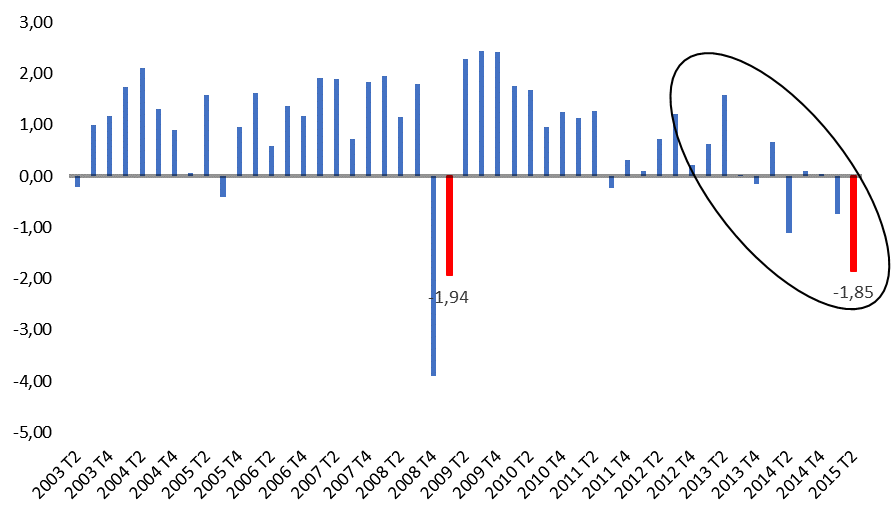
\includegraphics[width=.7\textheight]{PIB_Dessaz.png}
		\caption*{\textbf{Fonte:} IBGE, elaboração própria.}
	\end{center}
\end{figure}


%% Colocar série temporal do PIB
		% Objetivo: gráfico gerado no ggplot2
		% Colocar desemprego?
		% Incluir crise

No gráfico \ref{graf}, podem ser observados alguns momentos de inflexão importantes. O primeiro deles (A) registra os impactos da crise financeira internacional sobre a economia brasileira. Já o segundo (B) indica o começo da desaceleração econômica. O último deles (C) reflete a tímida retomada ensaiada recentemente (2016-7).


\begin{figure}[htb]
	\begin{center}
		\caption{Variação do PIB trimestral em comparação ao mesmo período do ano passado deflacionado pelo IPCA - (2001-2017)}
		\label{graf}
		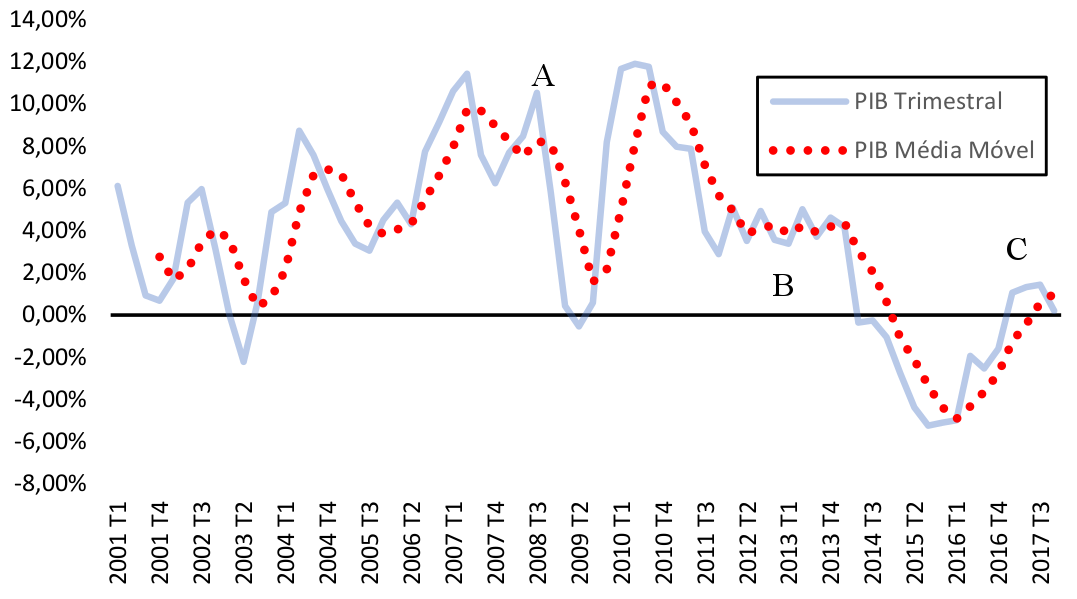
\includegraphics[width=.7\textheight]{PIB_FAPESP.png}
		\caption*{\textbf{Fonte:} IBGE, elaboração própria.}
	\end{center}
\end{figure}

% Colocar pontos no gráfico para referenciar no texto.

Essa datação apresentada guiará o projeto de pesquisa aqui elaborado. Os esforços serão endereçados para a compreensão do segundo desses pontos de inflexão. A relevância desta pesquisa, por outro lado, é observada no último ponto acima destacado. 



Portanto, o presente projeto é de suma importância para entender dois eventos correlatos, qual seja: (i) as causas da desaceleração e (ii) as possibilidades da retomada. Compreendido o por\-quê desta pesquisa, a seção seguinte tratará forma que será elaborada.








{\let\clearpage\relax \chapter{Metodologia}\label{Metodo}}




\section{Estrutura da dissertação}

A dissertação de mestrado que tem como base o presente projeto será dividida em duas partes. A primeira delas tem como objetivo identificar e responder as questões pontuadas na seção \ref{OBJ} deste documento, ou seja, tratar da discussão em torno dos limites do padrão de crescimento desenvolvimentista.  

No primeiro capítulo desta parte, serão abordadas as mudanças estruturais. Adiante, no capítulo 3, serão elencadas as características institucionais do Brasil e como podem interferir no desempenho econômico do país. No capítulo seguinte, serão arrolados os limites do lado da oferta e da demanda. 

 A segunda parte, por sua vez, tem como fim apresentar uma proposta de análise do período investigado na primeira parte. Isso será feito a partir da metodologia SFC pós-keynesiana. Para atingir este objetivo, um primeiro capítulo irá expor os elementos tanto da escola pós-keynesiana quanto da metologia SFC contrapondo-os com os modelos ortodoxos. 
 
 Tendo este referencial teórico em mãos, passar-se-á para a elaboração de um modelo SFC que pretende discutir: (i) inclusão financeira considerando as diferentes classes socioeconômicas;  (ii) políticas de ganhos salariais reais; (iii) regime de metas para a inflação; (iv) mudanças nos parâmetros comportamentais.
 
 Apesar das diferenças entre as partes, há um fio condutor que as ligam: compreender quais os limites do padrão de crescimento desenvolvimentista foram atingidos. 
 Portanto, a primeira parte da dissertação irá contemplar tais limites enquanto a segunda tratará desses mesmos temas a partir de outro prisma metodológico (modelagem). Entendida a estrutura que guiará este projeto, a seção seguinte apresenta os passos necessários para que seja executável.
 






\section{Passos metodológicos}\label{passos}

Como visto anteriormente, o presente projeto tem como base duas frentes de análise distintas explicitadas pela divisão em duas partes. Apesar dessas diferenças metodológicas, existem semelhanças entre as etapas que serão realizadas. Como consequência, uma parcela significativa das atividades a serem desenvolvidas tratarão simultaneamente de ambas as partes.

Feito essa ressalva, segue-se para o detalhamento das fases do projeto. No início do programa, será feita uma revisão bibliográfica que abrangerá os textos referentes à parte I e II da dissertação. 
Tendo em vista a quantidade de material a ser examinado, essa atividade demandará mais tempo de pesquisa (Ver tabela \ref{crono}).

Ao mesmo tempo, serão feitas pesquisas e aplicações de linguagem de programação para seguir com a proposta pretendida na parte II. Neste caso, a linguagem de programação a ser estudada é o R (Ver seção \ref{relev}) e a partir dele serão feitas as simulações e análise dos dados coletados.
%%% Como citar R?


Tais dados serão coletados das mais distintas bases e serão fundamentais para consolidar os argumentos apresentados nas duas partes do projeto. Além disso, é a partir dos dados coletados que se baseará parte das simulações feitas na segunda parte da dissertação. Sendo assim, a coleta dos dados e as simulações serão feitas em um período de tempo próximo em que a revisão bibliográfica esteja em um estágio mais avançado.

Já com relação às simulações, serão feitas a partir do momento que modelo SFC-PK esteja consolidado. Desse modo, a realização dessas simulações só será factível com o domínio da referida linguagem de programação (R). Por conta disso, esta etapa será elaborada em um estágio mais avançado do projeto.

Por fim, tendo os resultados em mãos, prosseguir-se-á para a análise dos dados e respectivas comparações com a literatura examinada na primeira etapa do projeto. Adiante, será realizada a descrição dos resultados obtidos. Com isso, conclui-se tanto a análise empírica quanto computacional dos dados.

Consequentemente, cumprindo as etapas elencadas anteriormente,  é possível realizar a redação da dissertação propriamente dita. Feitos esses passos, concluí-se o presente projeto atingindo os objetivos almejados. Essa seção, portanto, tratou dos passos metodológicos a serem seguidos, a seção seguinte, por sua vez, fará uma breve revisão de literatura.



{\let\clearpage\relax \chapter{Revisão bibliográfica}\label{Rev}}

Abordar:

\begin{itemize}
 \item Ótica da demanda e da produção para fazer um gancho com os objetivos do projeto
 \item Falar sobre alguns textos que discutem a desaceleração dos governos Dilma 1 e 1.5
 \item Interconectar com o que foi dito no projeto
 \item Fazer uma \textbf{breve} (!) introdução à metodologia SFC
 	\begin{itemize}
 		\item Aproveitar monografia
 			\begin{itemize}
				\item Como citar minha monografia? O.o
 			\end{itemize}
 	\end{itemize}
 \item Ponte para seção seguinte
\end{itemize}

O PIB de uma economia pode ser calculado a partir de três óticas: (i) renda, (ii) produção e (iii) demanda. 



%%% Falar sobre fronteira do sfc

{\let\clearpage\relax \chapter{Elementos relevantes do projeto}\label{relev}}

% Falar da importância e como este projeto está na fronteira

%\section{Simulação computacional}
%
%O uso de simulação computacional vem contribuindo para a análise de modelos econômicos mais sofisticados. A partir de processamento de dados  é possível avançar na avaliação de determinado modelo dinâmico levando em consideração diversos cenários. Desse modo, 

\section{Rotinas de programação em economia}

 Em economia, é comum o uso de \textit{softwares} dedicados à determinadas tarefas acadêmicas. No entanto, cada vez mais são utilizadas linguagens de programação nas mais diferentes áreas de conhecimento. O desenvolvimento de rotinas de programação possibilita uma maior autonomia do pesquisador para resolver problemas específicos e assim avançar na linha de pesquisa. Além disso, a distribuição dos programas criados pode contribuir para o avanço de outras fronteiras de pesquisa de forma mais difusa.
 
 Desse modo,  ao desenvolver um modelo macrodinâmico partindo de uma linguagem de programação, esse projeto de pesquisa pode auxiliar mais pesquisadores em suas investigações. Neste caso, optou-se por uma linguagem voltada para \textit{data science}: R \cite{RSoftware}. Vale notar que também é uma linguagem apropriada para  análise estatística e, portanto,  de grande valia para estudos na área de economia.

\section{Avanço na fronteira de pesquisa heterodoxa}

Por estar na fronteira de pesquisa, a metodologia SFC está em constante mudança. Em outras palavras, para responder muitas das questões que esta metodologia propõe é preciso avançar em termos de instrumental teórico. Desse modo, ao incluir elementos ainda não explorados dessa metodologia, esta pesquisa pode auxiliar no avanço da fronteira. 

Além disso, como visto na seção \ref{Rev}, esta metodologia é capaz de acomodar as mais variadas escolas de pensamento econômico. No entanto, será adotada uma perspectiva heterodoxa. Como consequência, este projeto pode ser uma frente de avanço na constituição de um programa de pesquisa heterodoxo mais consolidado. 
%Mais especificadamente, a linha teórica a ser seguida é a Pós-Keynesiana, 



{\let\clearpage\relax \chapter{Cronograma das atividades}\label{cronograma}}

A tabela \ref{crono} apresenta um esboço das atividades a serem desempenhadas ao longo desta pesquisa. Como a dissertação será desenvolvida junto das obrigações institucionais do programa de Mestrado, optou-se por incluir uma linha referente aos créditos das disciplinas que serão cursadas. Dito isso, segue abaixo o cronograma mencionado\footnote{Importante notar também que os itens 1-4 da tabela \ref{crono} dizem respeito aos passos metodológicos discutidos na Seção \ref{passos}.
}:

% Please add the following required packages to your document preamble:
% \usepackage{multirow}
% \usepackage{graphicx}
%\begin{table}[htb]
%	\centering
%	\caption{Cronograma de atividades}
%	\label{crono}
%	\resizebox{\textwidth}{!}{%
%		\begin{tabular}{|l|l|l|l|l|l|l|l|l|}
%			\hline
%			\multicolumn{1}{|c|}{} & \multicolumn{8}{c|}{Período} \\ \cline{2-9} 
%			\multicolumn{1}{|c|}{\multirow{-2}{*}{Atividade}} & \multicolumn{1}{c|}{0-3} & \multicolumn{1}{c|}{3-6} & \multicolumn{1}{c|}{6-9} & \multicolumn{1}{c|}{9-12} & \multicolumn{1}{c|}{12-15} & \multicolumn{1}{c|}{15-18} & \multicolumn{1}{c|}{18-21} & \multicolumn{1}{c|}{21-24} \\ \hline
%			\textbf{1. Fundamentação teórica} &\cellcolor[HTML]{FE0000}  & \cellcolor[HTML]{FE0000} & \cellcolor[HTML]{FE0000} & \cellcolor[HTML]{FE0000} & \cellcolor[HTML]{FE0000} & \cellcolor[HTML]{FE0000} & \cellcolor[HTML]{FE0000} &  \\ \hline
%			1.1. Disciplinas &  \cellcolor[HTML]{9B9B9B} & \cellcolor[HTML]{9B9B9B} & \cellcolor[HTML]{9B9B9B}  & \cellcolor[HTML]{9B9B9B}  &\cellcolor[HTML]{9B9B9B}  & \cellcolor[HTML]{9B9B9B} &  &  \\ \hline
%			1.2. Revisão bibliográfica & \cellcolor[HTML]{9B9B9B} &\cellcolor[HTML]{9B9B9B}  &\cellcolor[HTML]{9B9B9B}  & \cellcolor[HTML]{9B9B9B} &  &  &  &  \\ \hline
%			\textbf{2. Análise computacional} & \cellcolor[HTML]{FE0000} & \cellcolor[HTML]{FE0000} & \cellcolor[HTML]{FE0000} & \cellcolor[HTML]{FE0000} & \cellcolor[HTML]{FE0000} &\cellcolor[HTML]{FE0000}  &  &  \\ \hline
%			2.1. Pesquisa em linguagem de programação   & \cellcolor[HTML]{9B9B9B} & \cellcolor[HTML]{9B9B9B} & \cellcolor[HTML]{9B9B9B} & \cellcolor[HTML]{9B9B9B} & \cellcolor[HTML]{9B9B9B} &  &  &  \\ \hline
%			2.2. Construção do modelo teórico &  &  &  & \cellcolor[HTML]{9B9B9B} & \cellcolor[HTML]{9B9B9B} & \cellcolor[HTML]{9B9B9B} &  &  \\ \hline			
%			\textbf{3. Análise empírica} &  &  &  &  & \cellcolor[HTML]{FE0000} & \cellcolor[HTML]{FE0000} & \cellcolor[HTML]{FE0000} &  \\ \hline
%			3.1. Coleta de dados &  &  &  &  & \cellcolor[HTML]{9B9B9B} & \cellcolor[HTML]{9B9B9B} &  &  \\ \hline
%			3.2. Simulações &  &  &  &  &  & \cellcolor[HTML]{9B9B9B} & \cellcolor[HTML]{9B9B9B} &  \\ \hline
%			\textbf{4. Análise dos resultados} &  &  &  &  &  &\cellcolor[HTML]{FE0000}  & \cellcolor[HTML]{FE0000} &  \\ \hline
%			4.1. Comparações com a literatura &  &  &  &  &  & \cellcolor[HTML]{9B9B9B} & \cellcolor[HTML]{9B9B9B} &  \\ \hline
%			4.2. Descrição dos resultados obtidos &  &  &  &  &  &  & \cellcolor[HTML]{9B9B9B} &  \\ \hline
%			\textbf{5. Exame de qualificação} &  &  &  &  &  &  & \cellcolor[HTML]{009901} &  \\ \hline
%			\textbf{6. Redação da Dissertação de Mestrado} &  &  &  &  & \cellcolor[HTML]{FE0000} & \cellcolor[HTML]{FE0000} & \cellcolor[HTML]{FE0000} &  \\ \hline
%			\textbf{7. Defesa} &  &  &  &  &  &  &  & \cellcolor[HTML]{009901} \\ \hline
%		\end{tabular}%
%	}
%\end{table}



\begin{table}[H]
\centering
\caption{Cronograma de atividades}
\label{crono}
\resizebox{\textwidth}{!}{%
\begin{tabular}{|l|l|l|l|l|l|l|l|l|}
\hline
\multicolumn{1}{|c|}{} & \multicolumn{8}{c|}{Período} \\ \cline{2-9} 
\multicolumn{1}{|c|}{\multirow{-2}{*}{Atividade}} & \multicolumn{1}{c|}{0-3} & \multicolumn{1}{c|}{3-6} & \multicolumn{1}{c|}{6-9} & \multicolumn{1}{c|}{9-12} & \multicolumn{1}{c|}{12-15} & \multicolumn{1}{c|}{15-18} & \multicolumn{1}{c|}{18-21} & \multicolumn{1}{c|}{21-24} \\ \hline
\textbf{1. Fundamentação teórica} &  &  &  &  &   &  & &  \\ \hline
1.1. Disciplinas &  \cellcolor[HTML]{9B9B9B} & \cellcolor[HTML]{9B9B9B} & \cellcolor[HTML]{9B9B9B}  & \cellcolor[HTML]{9B9B9B}  &\cellcolor[HTML]{9B9B9B}  & \cellcolor[HTML]{9B9B9B} &  &  \\ \hline
1.2. Revisão bibliográfica & \cellcolor[HTML]{9B9B9B} &\cellcolor[HTML]{9B9B9B}  &\cellcolor[HTML]{9B9B9B}  & \cellcolor[HTML]{9B9B9B} & \cellcolor[HTML]{9B9B9B} &  &  &  \\ \hline
\textbf{2. Análise computacional} &  &  &  &  &  &  &  &  \\ \hline
2.1. Pesquisa em linguagem de programação   & \cellcolor[HTML]{9B9B9B} & \cellcolor[HTML]{9B9B9B} & \cellcolor[HTML]{9B9B9B} & \cellcolor[HTML]{9B9B9B} & \cellcolor[HTML]{9B9B9B} &  &  &  \\ \hline
2.2. Construção do modelo teórico &  &  &  & \cellcolor[HTML]{9B9B9B} & \cellcolor[HTML]{9B9B9B} & \cellcolor[HTML]{9B9B9B} &  &  \\ \hline			
\textbf{3. Análise empírica} &  &  &  &  &  &  &  &  \\ \hline
3.1. Coleta de dados &  &  &  &  & \cellcolor[HTML]{9B9B9B} & \cellcolor[HTML]{9B9B9B} &  &  \\ \hline
3.2. Simulações &  &  &  &  &  & \cellcolor[HTML]{9B9B9B} & \cellcolor[HTML]{9B9B9B} &  \\ \hline
\textbf{4. Análise dos resultados} &  &  &  &  &  &  &  &  \\ \hline
4.1. Comparações com a literatura &  &  &  &  &  & \cellcolor[HTML]{9B9B9B} & \cellcolor[HTML]{9B9B9B} &  \\ \hline
4.2. Descrição dos resultados obtidos &  &  &  &  &  &  & \cellcolor[HTML]{9B9B9B} &  \\ \hline
\textbf{5. Exame de qualificação} &  &  &  &  &  &  & \cellcolor[HTML]{9B9B9B} &  \\ \hline
\textbf{6. Redação da Dissertação de Mestrado} &  &  &  &  & \cellcolor[HTML]{9B9B9B} & \cellcolor[HTML]{9B9B9B} & \cellcolor[HTML]{9B9B9B} &  \\ \hline
\textbf{7. Defesa} &  &  &  &  &  &  &  & \cellcolor[HTML]{9B9B9B} \\ \hline
\end{tabular}%
}
\end{table}


%O cronograma \ref{crono} também mostra os grupos de atividades a serem desempenhadas, são elas: (i) fundamentação teórica; (ii) Análise computacional; (iii) Análise empírica e (iv) Redação da dissertação de mestrado. O tempo previsto para a dedicação deste grupo de atividades está destacado em vermelho. Os retângulos verdes, por sua vez, representam as obrigações institucionais: (i) Exame de Qualificação e (ii) Defesa da dissertação.


%
%{\let\clearpage\relax
%\includepdf[pagecommand=\chapter{Bibliografia fundamental}, pages={5}]{Bibliografia_Fundamental.pdf}}
%{\let\clearpage\relax
%	\includepdf[ pagecommand={} , pages={6-8}]{Bibliografia_Fundamental.pdf}}

%-----
% Referências bibliográficas
%-----
%\addcontentsline{toc}{chapter}{\bibname}




{\let\clearpage\relax \chapter{Bibliografia}}



	\nocite{*}

{\let\clearpage\relax\printbibliography[title={Referências básicas}, keyword={Basico}]}

{\let\clearpage\relax\printbibliography[title={Referências bibliográficas}, keyword={Referenciado}]}




%-----
% Fim do documento
%-----
\end{document}